\documentclass[11pt, upma4paper, twoside, openany, parskip=half]{book}

\usepackage{graphicx,color}
\usepackage{amssymb, amsmath, array}
\usepackage{hyperref}     
\usepackage{enumitem}
\usepackage{float}
\usepackage{listings}
\usepackage{caption}
\usepackage{parcolumns}

% for draft
\usepackage{color}  
% end for draft

\begin{document}

% Example of title page for the projects carried out within DEDIS
% Copied from lasec 

% Simply include it in your mastex tex file: 
%        % Example of title page for the projects carried out within DEDIS
% Copied from lasec 

% Simply include it in your mastex tex file: 
%        % Example of title page for the projects carried out within DEDIS
% Copied from lasec 

% Simply include it in your mastex tex file: 
%        \input{cover}


% Updated October 2016


\newcommand{\logoepfl}[0]{
  \begin{center}
    
\includegraphics[width=4cm]{logo_epfl_coul.eps}
  \end{center}
  \vspace{0.3cm}
  \hrule
}
\newcommand{\project}[1]{
  \begin{center}
    \large{#1}
  \end{center}
  \vspace{1cm}
}
\newcommand{\department}[1]{
  \begin{center}
    \large{#1}
  \end{center}
}
\newcommand{\lab}[1]{
  \begin{center}
    \large{#1}
  \end{center}
}
\newcommand{\supervisor}[3]{
  \begin{center}
    \begin{normalsize}{
        \bf #1}\\#2\\#3
    \end{normalsize}
  \end{center}
}
\renewcommand{\author}[1]{
  \begin{center}
    \Large{#1}
  \end{center}
  \vspace{0.5cm}
}
\renewcommand{\title}[1]{
  \vspace{3cm}
  \begin{center}
    \huge{#1}
  \end{center}
  \vspace{1.7cm}
}
\renewcommand{\date}[2]{
  \begin{center}
    \normalsize{#1 #2}
  \end{center}
  \vspace{0.5cm}
}


\thispagestyle{empty}


% begin title page
  \logoepfl
  
  \title{Enhancing Debian Update Service}
  
  \author{Gaspard Zoss}
  \department{School of Computer and Communication Sciences}
  \lab{Decentralized and Distributed Systems lab}
  \project{Semester Project}
  
  \date{January}{2017}
	
	\begin{center}
	  	\begin{tabular}[t]{ccc}
		      \begin{tabular}[t]{p{3.0cm}}
			     \supervisor{Responsible}{Prof. Bryan Ford}{EPFL / DEDIS}
		      \end{tabular}&
		      \begin{tabular}[t]{p{3.0cm}}
			      \supervisor{Supervisor}{Eleftherios Kokoris Kogias}{EPFL / DEDIS}
			  \end{tabular}&
			  \begin{tabular}[t]{p{3.0cm}}
				  \supervisor{Supervisor}{Kirill Nikitin}{EPFL / DEDIS}
			  \end{tabular}
		\end{tabular}
	\end{center}

% end title page




% Updated October 2016


\newcommand{\logoepfl}[0]{
  \begin{center}
    
\includegraphics[width=4cm]{logo_epfl_coul.eps}
  \end{center}
  \vspace{0.3cm}
  \hrule
}
\newcommand{\project}[1]{
  \begin{center}
    \large{#1}
  \end{center}
  \vspace{1cm}
}
\newcommand{\department}[1]{
  \begin{center}
    \large{#1}
  \end{center}
}
\newcommand{\lab}[1]{
  \begin{center}
    \large{#1}
  \end{center}
}
\newcommand{\supervisor}[3]{
  \begin{center}
    \begin{normalsize}{
        \bf #1}\\#2\\#3
    \end{normalsize}
  \end{center}
}
\renewcommand{\author}[1]{
  \begin{center}
    \Large{#1}
  \end{center}
  \vspace{0.5cm}
}
\renewcommand{\title}[1]{
  \vspace{3cm}
  \begin{center}
    \huge{#1}
  \end{center}
  \vspace{1.7cm}
}
\renewcommand{\date}[2]{
  \begin{center}
    \normalsize{#1 #2}
  \end{center}
  \vspace{0.5cm}
}


\thispagestyle{empty}


% begin title page
  \logoepfl
  
  \title{Enhancing Debian Update Service}
  
  \author{Gaspard Zoss}
  \department{School of Computer and Communication Sciences}
  \lab{Decentralized and Distributed Systems lab}
  \project{Semester Project}
  
  \date{January}{2017}
	
	\begin{center}
	  	\begin{tabular}[t]{ccc}
		      \begin{tabular}[t]{p{3.0cm}}
			     \supervisor{Responsible}{Prof. Bryan Ford}{EPFL / DEDIS}
		      \end{tabular}&
		      \begin{tabular}[t]{p{3.0cm}}
			      \supervisor{Supervisor}{Eleftherios Kokoris Kogias}{EPFL / DEDIS}
			  \end{tabular}&
			  \begin{tabular}[t]{p{3.0cm}}
				  \supervisor{Supervisor}{Kirill Nikitin}{EPFL / DEDIS}
			  \end{tabular}
		\end{tabular}
	\end{center}

% end title page




% Updated October 2016


\newcommand{\logoepfl}[0]{
  \begin{center}
    
\includegraphics[width=4cm]{logo_epfl_coul.eps}
  \end{center}
  \vspace{0.3cm}
  \hrule
}
\newcommand{\project}[1]{
  \begin{center}
    \large{#1}
  \end{center}
  \vspace{1cm}
}
\newcommand{\department}[1]{
  \begin{center}
    \large{#1}
  \end{center}
}
\newcommand{\lab}[1]{
  \begin{center}
    \large{#1}
  \end{center}
}
\newcommand{\supervisor}[3]{
  \begin{center}
    \begin{normalsize}{
        \bf #1}\\#2\\#3
    \end{normalsize}
  \end{center}
}
\renewcommand{\author}[1]{
  \begin{center}
    \Large{#1}
  \end{center}
  \vspace{0.5cm}
}
\renewcommand{\title}[1]{
  \vspace{3cm}
  \begin{center}
    \huge{#1}
  \end{center}
  \vspace{1.7cm}
}
\renewcommand{\date}[2]{
  \begin{center}
    \normalsize{#1 #2}
  \end{center}
  \vspace{0.5cm}
}


\thispagestyle{empty}


% begin title page
  \logoepfl
  
  \title{Enhancing Debian Update Service}
  
  \author{Gaspard Zoss}
  \department{School of Computer and Communication Sciences}
  \lab{Decentralized and Distributed Systems lab}
  \project{Semester Project}
  
  \date{January}{2017}
	
	\begin{center}
	  	\begin{tabular}[t]{ccc}
		      \begin{tabular}[t]{p{3.0cm}}
			     \supervisor{Responsible}{Prof. Bryan Ford}{EPFL / DEDIS}
		      \end{tabular}&
		      \begin{tabular}[t]{p{3.0cm}}
			      \supervisor{Supervisor}{Eleftherios Kokoris Kogias}{EPFL / DEDIS}
			  \end{tabular}&
			  \begin{tabular}[t]{p{3.0cm}}
				  \supervisor{Supervisor}{Kirill Nikitin}{EPFL / DEDIS}
			  \end{tabular}
		\end{tabular}
	\end{center}

% end title page



\tableofcontents

\chapter{Introduction}
Software updates are an essential element in securing any software running on devices going from small embedded devices to computer clusters. In this project, we will study how security of software update process in large projects can be improved and apply it to Debian APT \cite{_apt_????}. 

When a new feature is added or when a bug is fixed in one of the software available through the Debian package manager, the package's maintainer, often one of the project's developers, generates a binary by compiling the code, hashes it and creates various scripts used to install, upgrade or remove the software. These scripts and the binary are then packed together and placed inside a repository, from which the end user may download the update. The repository itself is signed, usually using a single  private cryptographic key and the binaries are verified by using checksums. Additionally, the software can be made reproducible by the developers allowing users to verify if the given binary was produced using the publicly available source code. But as of today, not all Debian packages are reproducible \cite{_overview_????}.

The described system has multiple attacks vectors; first, if reproducible builds aren't used, a malicious developer could distribute a binary containing some spyware or hidden functionality not present in the public code repository without informing the user and sign the binary with his private key. Then, the end-user's only choice would be to trust the package maintainer and the only certitude he has is that the binary he received is the one he was intended to receive. Secondly, even if the package maintainer is assumed to be trusted, a powerful third party opponent could steal the maintainer's private key and sign a modified binary which he could then substitute without noticing the end-user. The single signing key is thus a single point of failure in this architecture.

On the other hand, even if reproducible builds are available for a given package not all code details are monitored and each end-user should review every parts of the code to have the absolute certainty that the binary is safe. Furthermore, reproducing a package may take a lot of time, for example it takes on average 32 hours to build Tor on a modern laptop \cite{_tor_????}, and most end-users don't want to spend time on reproducing packages.

We propose a new way of verifying Debian update by introducing a wrapper around \emph{APT} that verifies the validity of the updates against a public cothority service that keeps an updated \emph{log} of the Debian updates on a per-repository basis.

First, we will present the background in a first part. Then we will present the main ideas of a Collectively Signed APT and describe the Debian release system in the second part. In the third part, we will discuss our implementation and, in the fourth part, how we evaluated the results. Finally we will discuss the future work and formulate a conclusion.

\section{Background}
Aside of introducing \textsc{Chainiac}, a decentralized software-update framework \cite{_back_2016}, authors also propose to extend it to large projects. They built \textsc{Chainiac} on top of \textsc{CoSI}, a scalable witness cosigning protocol \cite{syta_keeping_2015}. They introduce the concept of \emph{skipchains}, a data structure built by combining ideas from blockains and skiplists. Such \emph{skipchains} are useful as a way of maintaining a traversable public log of all updates for a given software. 

A \emph{skipchain} enables the client to traverse the timeline in both backward and forward direction, by, in the case of backward links, including a cryptographic hash of the previous block to the current one (similar as the blockchain case) and, in the case of forward links, a cryptographic signature of future blocks is retroactively appended to the previous block. Additionally, \emph{skipchains}' blocks have links to several other blocks to enable a faster traversal. The height of the \emph{skipchain} determines the number of links and how far the backward and forward links are going.

These \emph{skipchains} constitute a public log and they are maintained by a \textsc{Cothority}, a decentralized collective authority. This \textsc{Cothority} consists of an arbitrary number of hosts that exchanges informations via various protocols and runs custom services on each hosts.

\chapter{Collectively Signed APT}

\section{The Debian release system}
As Debian is under continual development, the repositories organization is carefully crafted in a way that enables every user to get updates as frequently as he desires. For example, the administrator of a server used in production may want to update the packages only when the update is really necessary as it fixes a major security vulnerability or when the update has been successfully tested and is safe to deploy on a production server. On the opposite, a developer may want to receive the latest updates as soon as they are available, even if a few bugs are still present.

To tackle with these very different requirements, the Debian community has separated the repositories into various categories; The \emph{stable} release with major version approximately every two years and minor versions, called Point Release, every few months. On top of that, \emph{stable-update} gives early access to updates which will be added to the next Point Release for some softwares that have a much smaller release cycle, such as \emph{clamav} (an antivirus software) or the Linux kernel. Security-critical updates go through a different repository, \emph{stable/updates} on \emph{security.debian.org}, which enables the updates to be pushed to the user on the same day the update is released. This security-critical updates are then merged in the \emph{stable} release. The \emph{testing} release contains the latest version of the packages which is stable enough (i.e. the packages have to pass different automatic requirements). Additionally, the \emph{stable-proposed-updates} repository contains packages which are proposed for the next \emph{stable} release but are not fully tested yet. Figure~\ref{debian_repo_summary} shows the overall Debian repository structure.

\begin{figure}
\centering
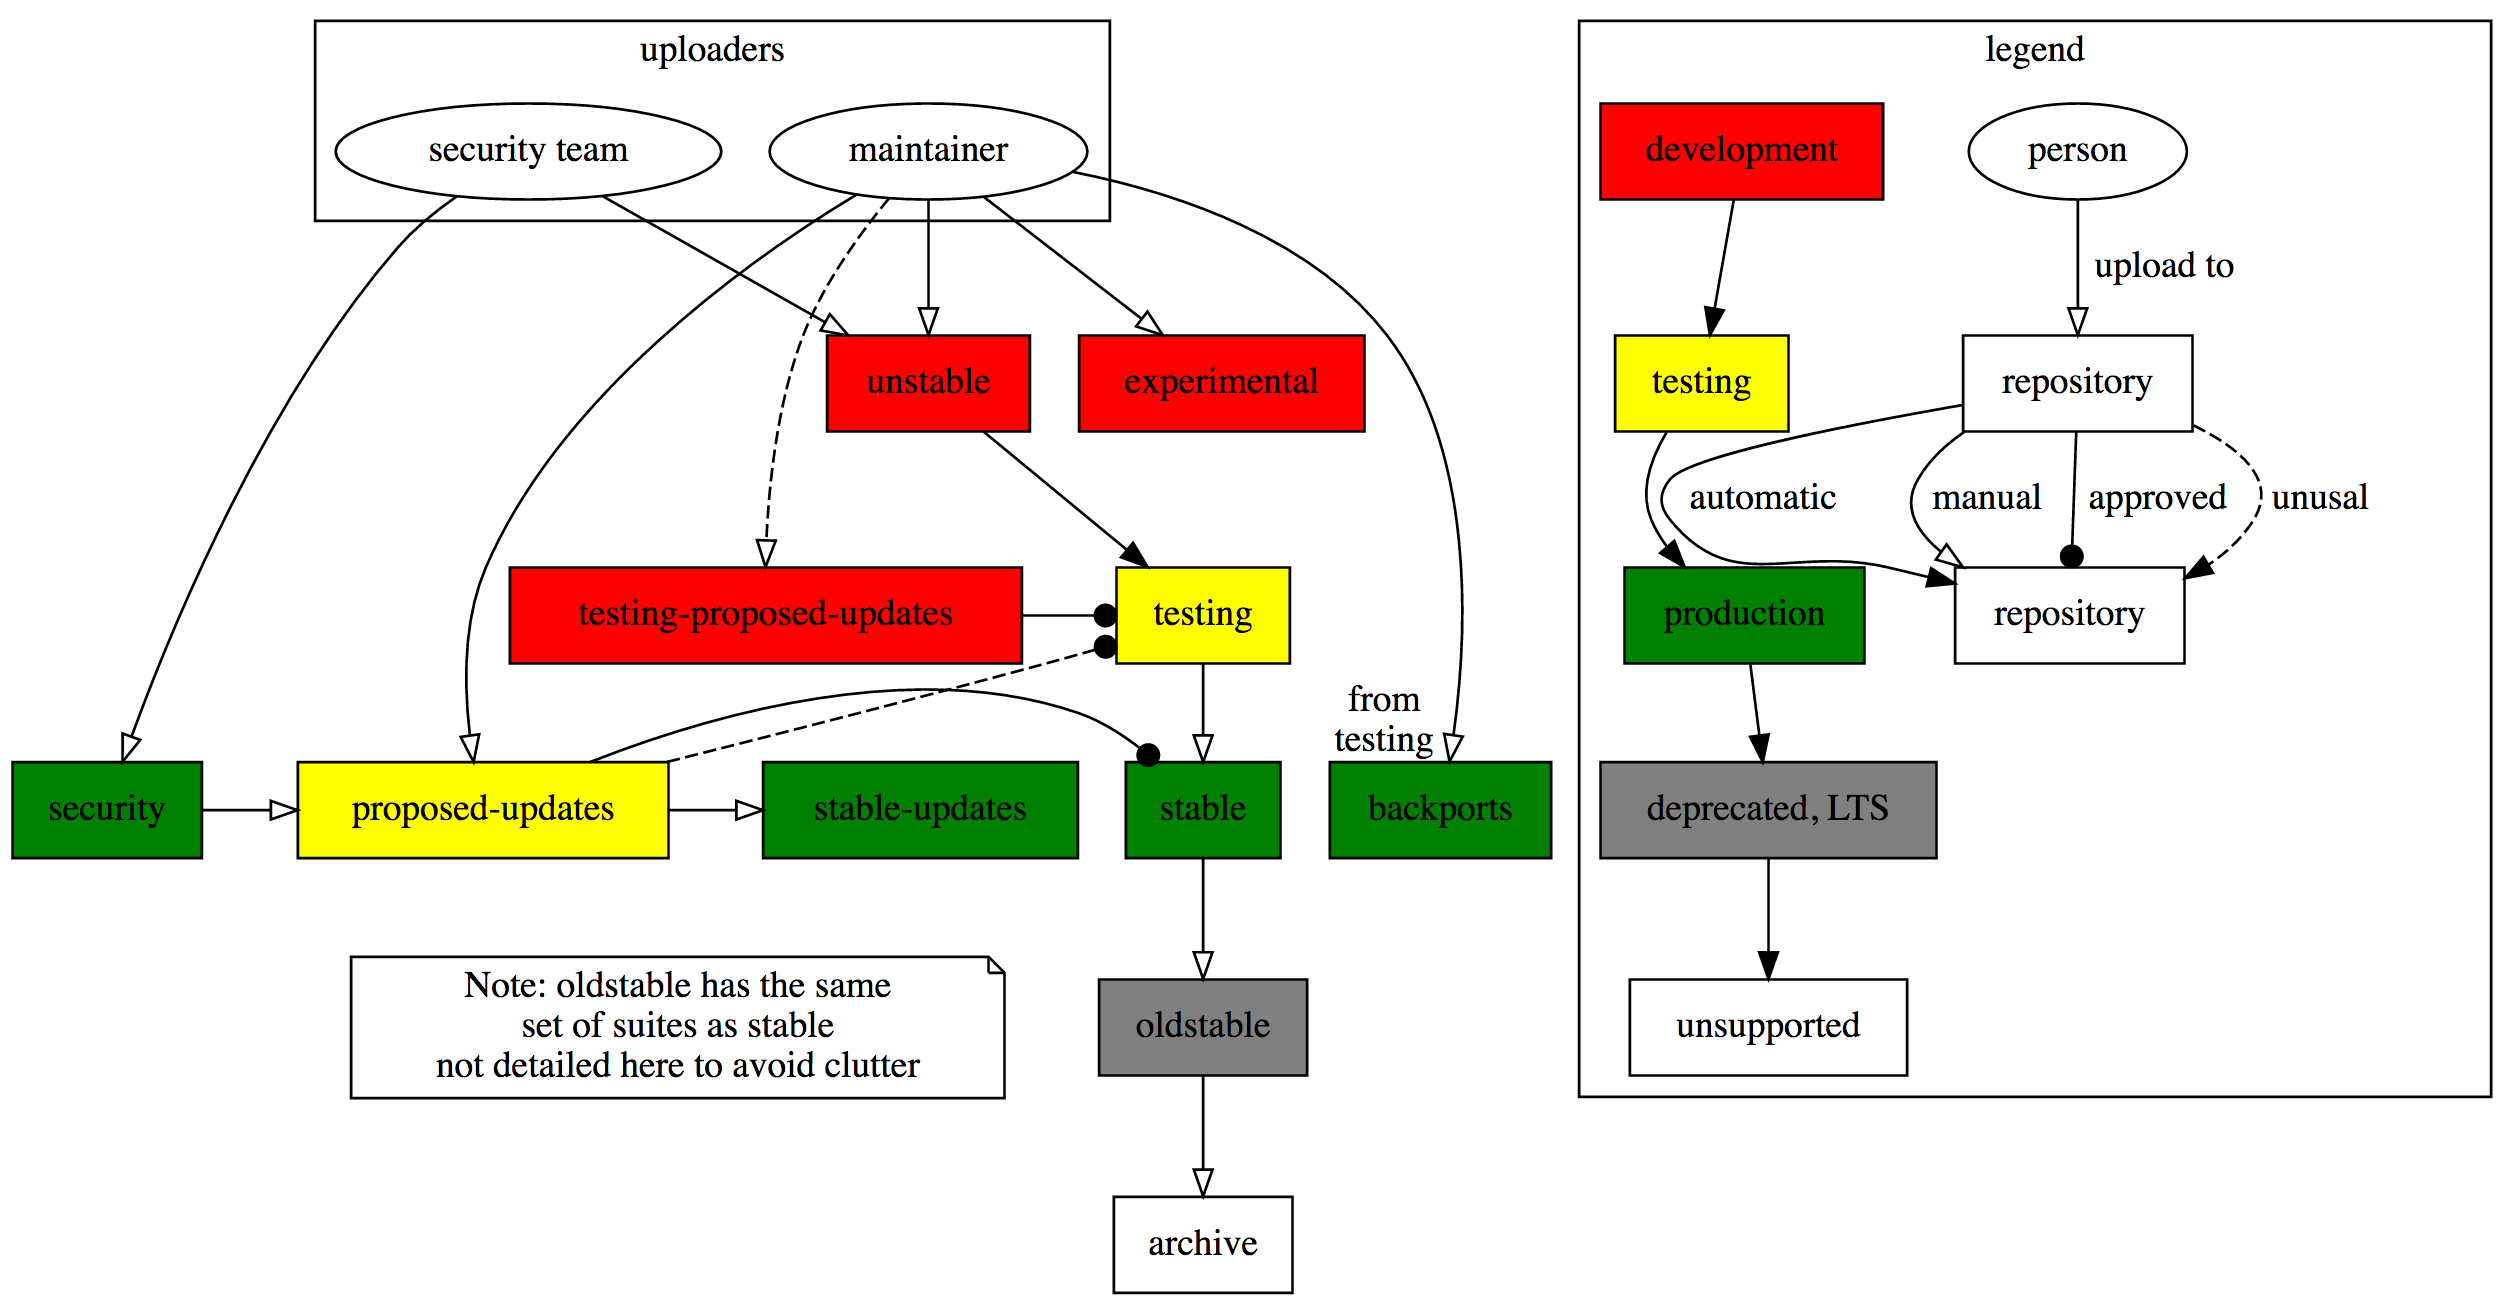
\includegraphics[width=400px]{debian_repo_summary.png}
\caption{Debian Repository Workflows \cite{debian_debianreleases_????}}
\label{debian_repo_summary}
\end{figure}

In this work, we will focus on the \emph{stable}, the \emph{stable-updates}, the \emph{testing} and the \emph{security} repositories, as these are the default way to receive updates on a standard installation of Debian. Adapting the project to other repositories will be discussed at the end of this document.

\subsection{Update frequency}

To ensure the feasibility of creating a skipchain per Debian repository we extracted statistics from the Debian Snapshot project \cite{_debian_????}. Table~\ref{repo_update_freq} summaries the update frequencies of packages from the various Debian repositories (only for \emph{binary-amd64}).

\begin{table}[h]
\centering
\begin{tabular}{ | l | c | }
\hline
repository & approximative update frequency \\
\hline
\emph{stable} (Point Release) & $2-3$ months \\
\emph{stable-update} & $1$ month \\
\emph{security} & $2$ days \\
\emph{testing} & less than $1$ day \\
\hline
\end{tabular}
\caption{Update frequencies for some of the Debian repositories}
\label{repo_update_freq}
\end{table}

We also looked at the number of packages updated per repository release, which are summarized in Table~\ref{repo_update_num_of_packages}
	
\begin{table}[h]
	\centering
	\begin{tabular}{ | l | c | }
		\hline
		repository & Average number of packages per release \\
		\hline
		\emph{stable} (Point Release) & $70$ \\
		\emph{stable-update} & $2$ \\
		\emph{security} & $3$ \\
		\emph{testing} & $100$ \\
		\hline
	\end{tabular}
	\caption{Average number of packages per release}
	\label{repo_update_num_of_packages}
\end{table}

	
\section{Collectively Signed Debian Update Service}

\subsection{Extending CHAINIAC}
\textsc{Chainiac} \cite{_back_2016} is a decentralized software-update framework working closely with \textsc{Cothorities} \cite{syta_keeping_2015}. Authors proposed a way to extend \textsc{Chainiac} to large projects. We study here the feasibility and efficiency of the proposed ideas, and design their implementation into Debian. Using this method could also enable a smooth transition from the actual state of Debian updates to a fully verified and reproducible update-framework.

Our implementation is composed of three distinct parts; a server part, running on a Cothority, responsible for maintaining the Debian skipchains, another server part used by the repository maintainers to track changes in the repository and to update corresponding skipchain and a client which is a modified version of \emph{APT} to verify updates before installing them.

\subsection{The Cothority and server parts}
The server part runs as a Cothority service. For each Debian update repository configured to do so, it \emph{maintains} a Skipchain where each block is the root of a \emph{Merkle tree}. This Merkle tree is formed by having the head of an individual package's skipchain as leaf (see Figure \ref{overall_skipchain} for the overall scheme). Additionally, some packages can be added to the repository Merkle tree even if they do not possess an individual Skipchain (for example during a transition period or if having a Skipchain for this package is not relevant). For those packages, the root of the Merkle-tree formed by its files hashes is added to the Repository Merkle tree instead of the latest Skipblock. This service is accessed by both the server and the client through an API. 

\begin{figure}[H]
	\centering
	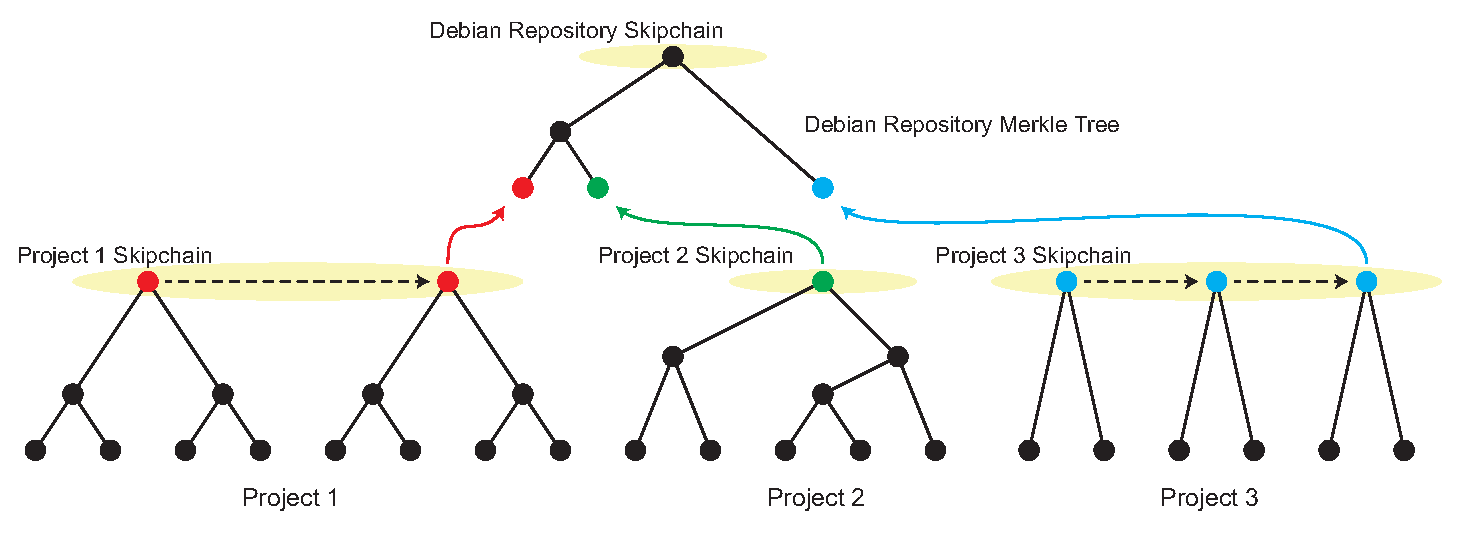
\includegraphics[width=380pt]{overall_skipchains}\vspace{-0pt}
	\caption{The big picture of a Skipchain for some Debian Repository and 3 fictional packages}
	\label{overall_skipchain}
\end{figure}

The server part which runs on the Debian repository maintainer's server is triggered multiple times per day by a cron job. Its main role is to request the latest's skipchain block from each individual package's software update service. After receiving all the replies, it aggregates all the data into a single message sent to the Debian Update Cothority service using an API. The later then creates a Merkle-tree from this aggregated answer by having packages' hashes as leaves in the tree. If the new root of this tree differs from the previous ones (which implies that some of the packages have changed), it is collectively signed and added to the Debian Update Skipchain. To ensure the information's freshness in the Debian Update Skipchain, \textsc{Chainiac}'s role-based trust delegation model is applied to the Debian Update project. In the case where a package doesn't have an individual Skipchain, the server part can also be configured to include some packages' hash in the aggregated answer by building a Merkle-tree of its files and including the root of this Merkle-tree in the Debian Update Skipchain.

\subsection{The user client part}
The client part is a modified version of the \emph{Advanced Packaging Tool} which verifies the downloaded update against a public Update Cothority. When the user wants to update its distribution, the \emph{APT} wrapper performs the following tasks :

\begin{enumerate}[noitemsep]
\item The wrapper calls \emph{apt-get update} to download the latest package lists and their headers.
\item It then requests the latest signed Skipblock from the Cothority's release skipchain.
\item After having downloaded the Skipblock, the wrapper verifies the signature of the block.
\item It then verifies the packages needed to be updated by computing the Merkle proof verification for each of them using the informations it received from the Cothority.
\item The wrapper then uses \emph{apt} to download the latest version of the packages that requires an upgrade but do not install them yet.
\item For each of the outdated packages installed, the client then goes to individual package's Skipchains and verify them individually using the method described in \textsc{Chainiac}.
\item On success, the client can be sure that the given package is the correct one and install it.
\end{enumerate}

\chapter{Implementation}
%\section{Problems that arose and solutions implemented to solve them}
%\section{Strategical choices undertaken during implementation}
We implemented the clients and the server in Go \cite{_go_????}. The following sub-sections describe their implementations and the strategical choices undertaken. Figure \ref{architecture} shows the general architecture described in the following sections.

\begin{figure}[H]
	\centering
	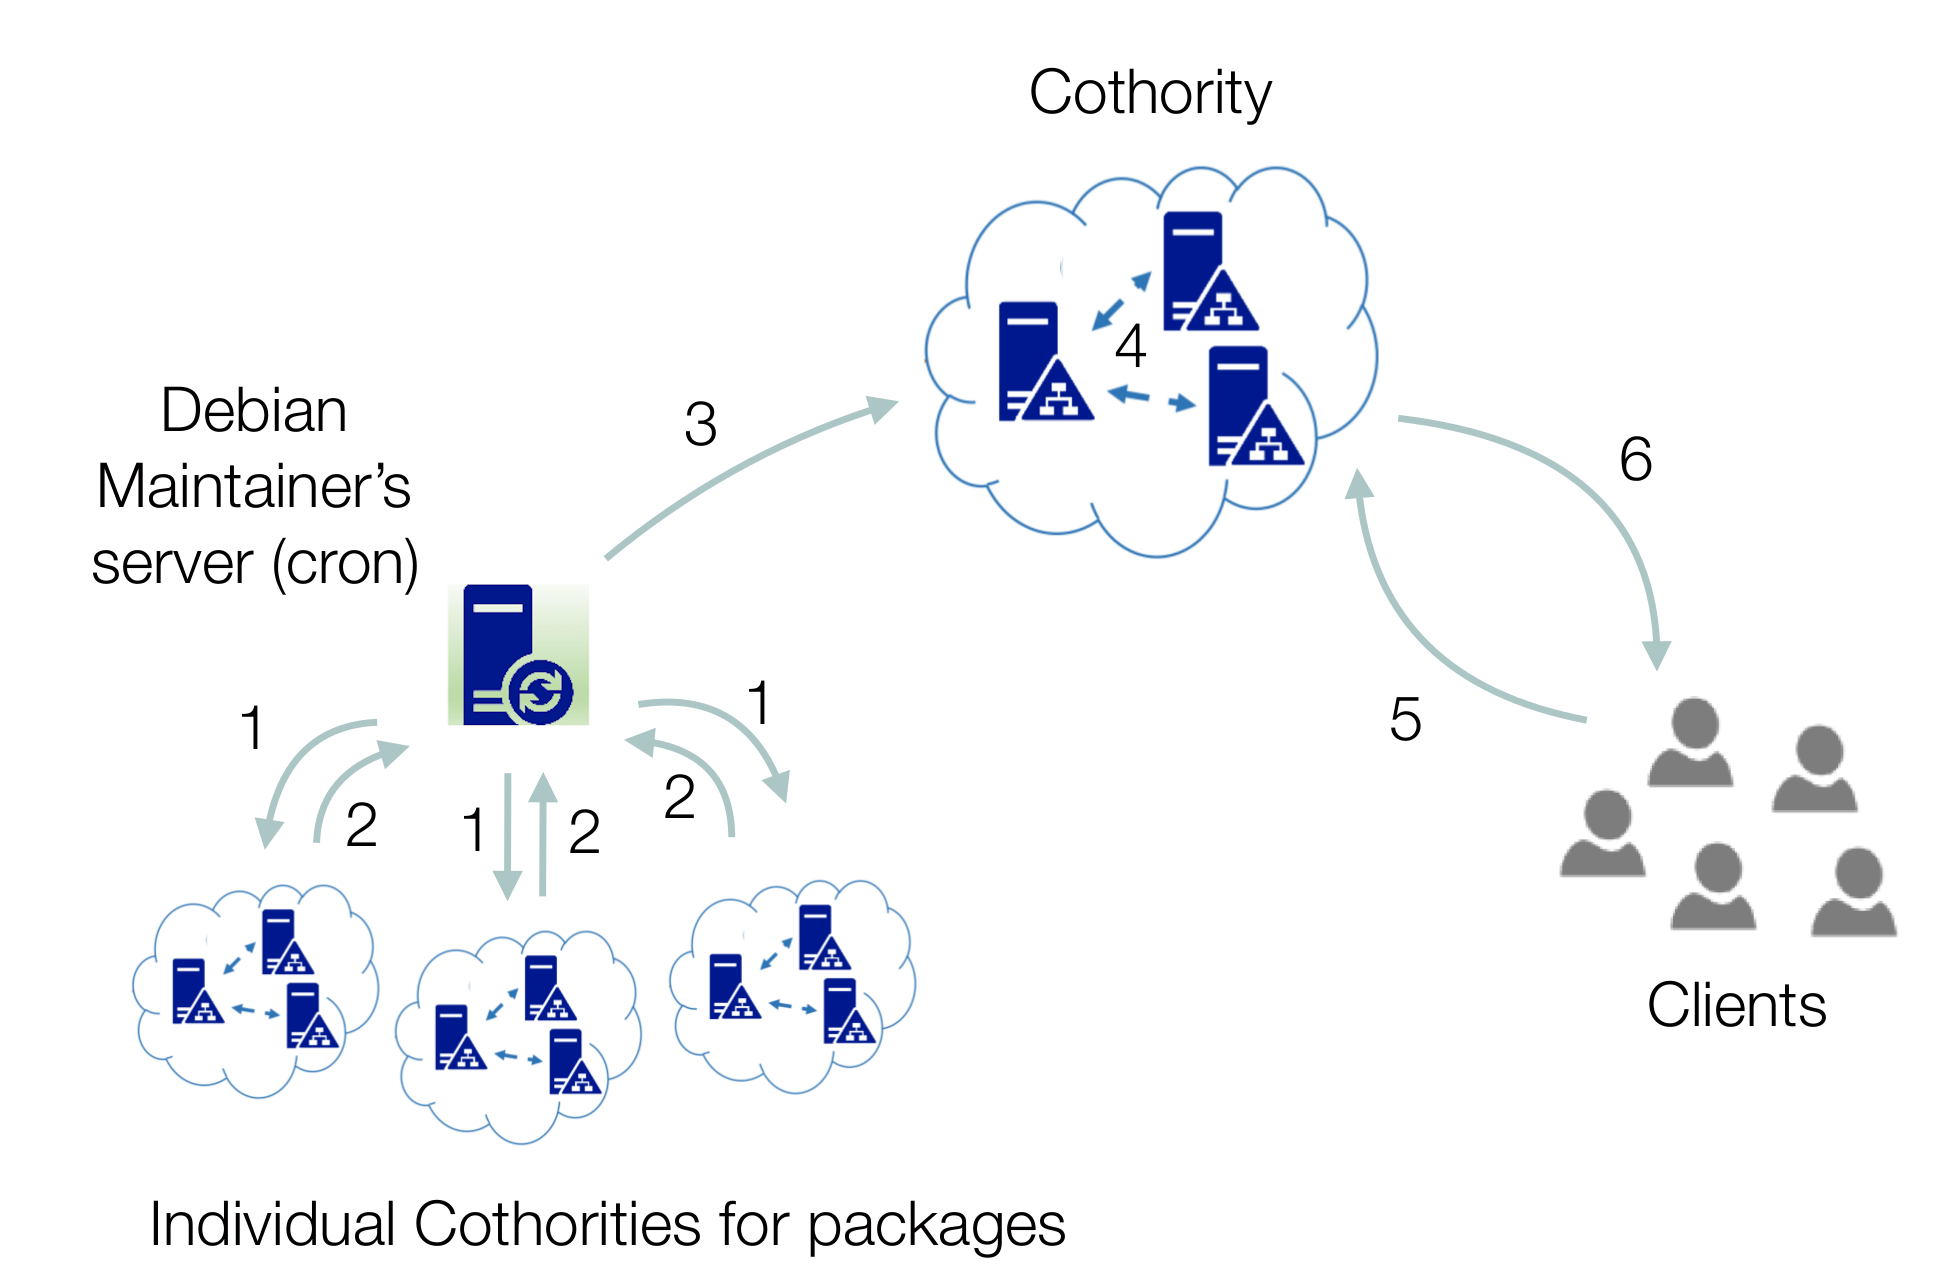
\includegraphics[width=330pt]{architecture.png}
	\caption{General architecture of the project. (1) are the latest block requests from the Maintainer's server to the individual Cothorities, (2) are the answers to those requests. (3) is the aggregated answer sent to the Debian Repository Cothority. (5) and (6) are the request and answer from the client to the Cothority.}
	\label{architecture}
\end{figure}

\section{The Cothority Service}
The Debian Update Cothority Service part follows closely the existing implementation of the Software Update Cothority Service with a few differences. Instead of having a service that maintains Skipchains on a per-package basis, our implementation now has a service that maintains Skipchains on a per-repository basis. To simulate the aggregated message received by the service, we decided to use Debian Snapshots \cite{_snapshot.debian.org_????} as an aggregated message to construct the Debian Repository Merkle-tree.

The first step for the Debian repository maintainer's server is to ask the service to create a new Skipchain for a given Snapshot. This is done by providing the service with the initial \emph{Release} file, which describes the repository name, version and various parameters and the initial \emph{Packages} file, which describes all the packages available at that time in the repository, their hashes, versions and other informations. To simplify the use of the service, we have chosen that both of those files are exactly the files downloaded from the Snapshot project without requiring any modifications. Alongside, other parameters are passed to the Cothority service, such as the skipchain parameters and the precomputed Merkle tree root and proof. The service then verifies this initial state by verifying the root of the Merkle tree against the proof. On successful verification, the service sends back the latest block of the Skipchain. Figure \ref{creation_messages} shows a simplified version of the request and answer to the service.


\begin{figure}[H]
\noindent\begin{minipage}[t]{.45\textwidth}
\begin{lstlisting}[frame=tlrb,basicstyle=\ttfamily]{Name}
CreateRepository  {
   Repository  
   RootID
   Proofs
   Base 
   Height 
}
\end{lstlisting}
\end{minipage}\hfill
\begin{minipage}[t]{.45\textwidth}
\begin{lstlisting}[frame=tlrb,basicstyle=\ttfamily]{Name}
CreateRepositoryReturn {
   LatestBlock
}
\end{lstlisting}
\end{minipage}
\caption{The informations sent and received on creation of a new Skipchain}
\label{creation_messages}
\end{figure}

When a new Debian Snapshot is produced, the Skipchain has to be updated with these new informations. When receiving new datas from the Debian maintainer's server, which consist of a repository new snapshot, the service first checks if some packages where updated or if the snapshot is the same as the previous one. Depending on the repository, the later case can happen often, for example the stable repository only had 13 changes during the past year. The service then updates the Timestamp Skipchain, even if the new Snapshot does not contain changes since the previous one, and updates the Data Skipchain only if the Snapshot is different than the previous one. The service then sends back the latest block of the Skipchain. Figure \ref{update_messages} shows a simplified version of the request and answer to the service.

\begin{figure}[H]
\noindent\begin{minipage}[t]{.45\textwidth}
\begin{lstlisting}[frame=tlrb,basicstyle=\ttfamily]{Name}
UpdateRepository  {
   LatestBlock
   Repository  
   RootID
   Proofs 
}
\end{lstlisting}
\end{minipage}\hfill
\begin{minipage}[t]{.45\textwidth}
\begin{lstlisting}[frame=tlrb,basicstyle=\ttfamily]{Name}
UpdateRepositoryRet {
   LatestBlock
}
\end{lstlisting}
\end{minipage}
\caption{The informations sent and received on update of the Skipchain}
\label{update_messages}
\end{figure}


\section{The server part}
Our prototype implementation of the Debian Repository maintainer's server part consists on a script which downloads the Debian Snapshots \cite{_snapshot.debian.org_????} (both the Package and Release files) given the name of the repo, a starting date and an ending date. Simulations then use these files and a Cothority's service API to create and update the Skipchains for each repository. These two files are parsed by the service and the relevant informations are stored in the Skipchain. Figure \ref{stored_skipchain} shows the datas extracted from the \emph{Package} and \emph{Release} files.

\begin{figure}[H]
\noindent\begin{minipage}[t]{.45\textwidth}
\begin{lstlisting}[frame=tlrb,basicstyle=\ttfamily]{Name}
Repository {
   Origin
   Suite 
   Version 
   []Packages
   SourceUrl
}
\end{lstlisting}
\end{minipage}\hfill
\begin{minipage}[t]{.45\textwidth}
\begin{lstlisting}[frame=tlrb,basicstyle=\ttfamily]{Name}
Packages {
   Name 
   Version
   Hash 
}
\end{lstlisting}
\end{minipage}
\caption{Datas extracted from the \emph{Release} and \emph{Package} files}
\label{stored_skipchain}
\end{figure}

\section{The client part}
While having a modified version of \emph{APT} would be a production ready software, we decided to implement a wrapper for \emph{APT} in Go. Doing so allows us to avoid re-implementing most of the networking and CoSi functions already available. Our wrapper handles the extra communication with the Cothority and the verification of the repository's state validity. It then performs calls to the installed \emph{APT} version. We took as an example the idea of \emph{yaourt} \cite{_piec/yaourt_????}, a \emph{pacman} \cite{_pacman_????} front end used by \emph{Arch Linux} users which adds the \emph{Arch User Repository}'s packages to \emph{pacman}. To simplify our simulation, this client was abstracted using only the API calls instead of launching the full client every time. When a client makes a request to the Cothority through the API, the service sends the latest Skipblock containing the signed root and a list of all the packages in the repository containing the package's hash and proofs. It then verifies the root's signature and can check the proof for all the installed packages.

\chapter{Results and Evaluation}
To evaluate our proposed solution, we used the simulation framework included in the \emph{Cothority} codebase. This framework allowed us to run the simulations on multiple platforms using the same code. We implemented various simulations to cover most of the test cases and thus extract various metrics. The following sections show the different simulations we ran using the \emph{localhost} simulation (as the simulations required only a limited CPU and memory power, we did not need to run them on DetherLab or Mininet).

\section{Cothority: Adding new release}
To test the CPU load on the Cothority depending on the number of packages in the repository added to the Skipchain, we implemented a simulation where a Cothority with 4 nodes is created, and a new release for a repository containing a certain number of packages was added to the Skipchain. Figure \ref{num_users} shows the average CPU time in second against the number of packages in the repository. Three metrics were individually measured; the time it took to verify the individual packages signatures (coming from each individual Cothority's Skipchains), in our test it was one single signature verification times the number of packages, the time it took to sign the root of the produced Merkle tree and the time it took to verify all the proofs from the individual packages. It is interesting to read on the graph that signing the root is nearly constant, as excepted and that both the proofs and signature verifications are linearly dependent on the number of packages.
\begin{figure}[H]
	\centering
	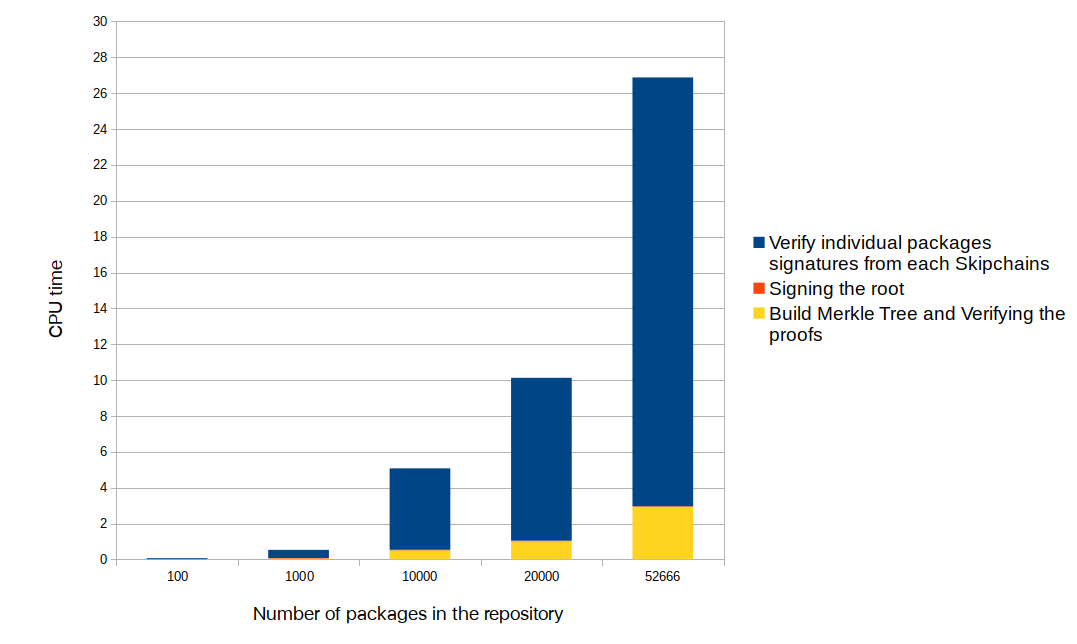
\includegraphics[width=300pt]{cothority_measures_lin.png}
	\caption{The CPU time usage in second against the number of packages in the repository.}
	\label{num_users}
\end{figure}

\section{Client: CPU usage}
In order to measure the additional load on the clients, we created a simulation where a client requests and verifies the latest block of the Skipchain and measured the average CPU time in seconds it took to verify the proofs and to verify the signatures. We included in the graph the time it took to verify a single GPG signature and the hashes for all those packages in \emph{APT} as a baseline. Figure \ref{num_packages_installed} shows the average CPU usage in second against the number of packages installed on the client machine. Again, this simulation was run with a Cothority of 4 nodes.


Computing the proofs on the client also depends on the number of packages in the repository in the Skipchain. We used subsets of the \emph{testing} repository with 1, 10, 100, 1000, 10000 and 52666 (the entire \emph{testing} repository) packages and measured the time it took to compute the proofs and to verify the signature. Figure \ref{num_package_in_repo} shows those metrics. Again, as a baseline we used the time it took for APT to run. This simulation was run with a 4 node Cothority.

\begin{figure}[H]
	\centering
	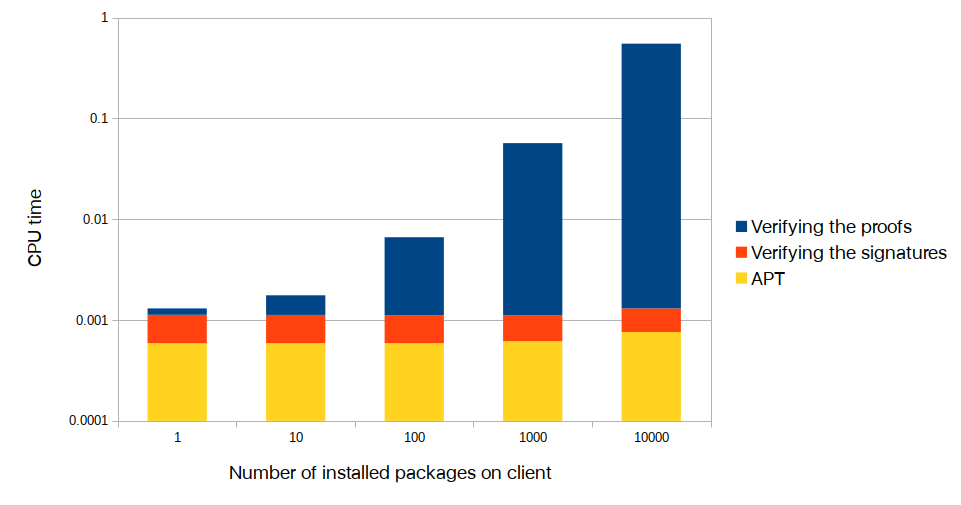
\includegraphics[width=300pt]{client_CPU_measures_num_packages.png}
	\caption{The average CPU time (in second) usage against the number of installed packages on a client.}
	\label{num_packages_installed}
\end{figure}

\begin{figure}[H]
	\centering
	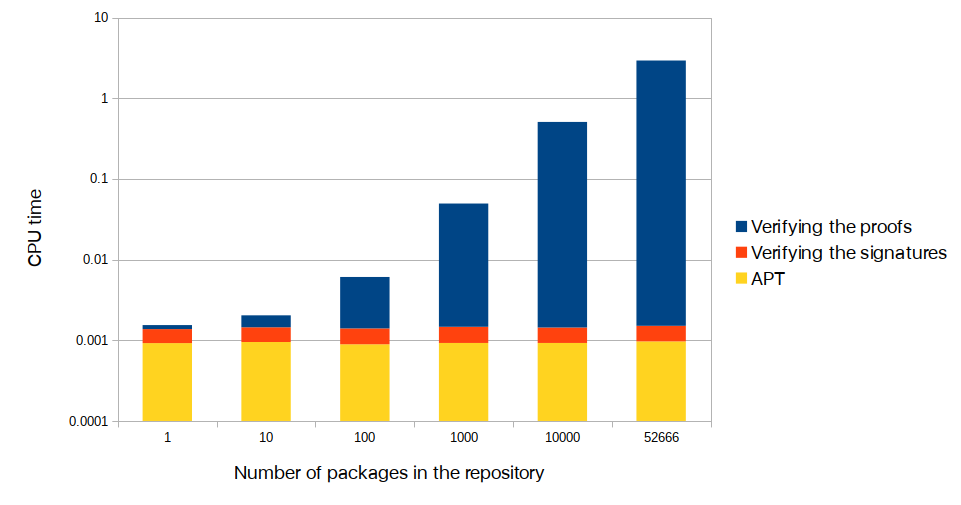
\includegraphics[width=300pt]{client_CPU_measures.png}
	\caption{The average CPU time (in second) usage against the number of packages in the repository.}
	\label{num_package_in_repo}
\end{figure}

\section{Client: Bandwidth usage}

Using the same setting to as in the later case to also measure the bandwidth overhead on the client compared to plain APT. This result is shown on figure \ref{num_package_in_repo_bandwidth}.

\begin{figure}[H]
	\centering
	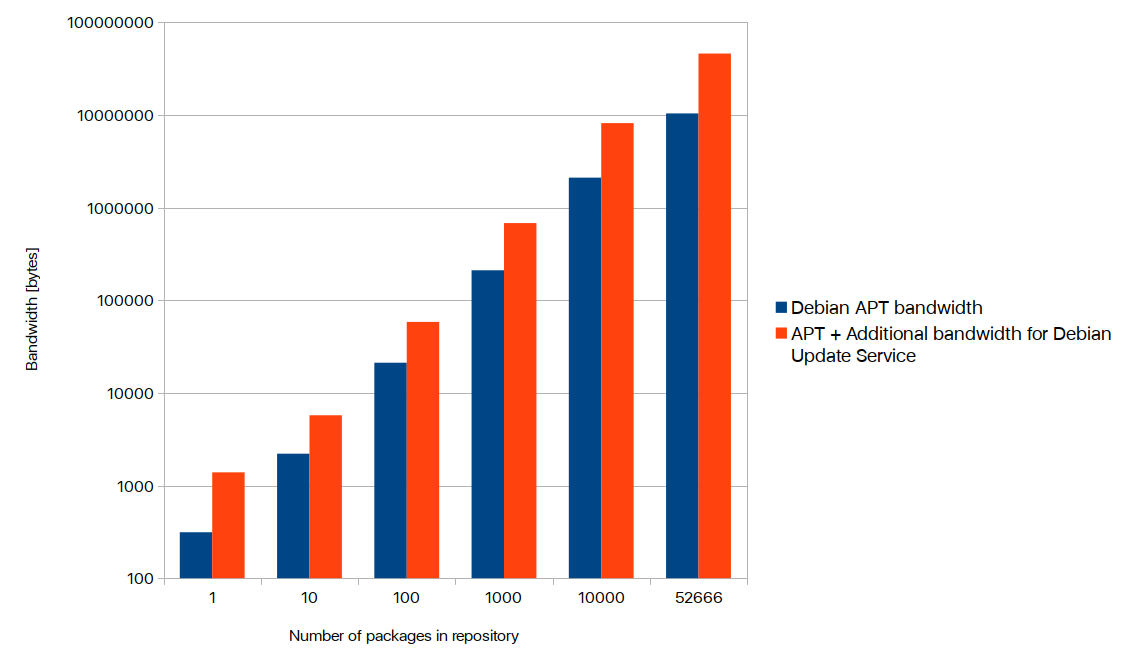
\includegraphics[width=300pt]{client_BW_measures.png}
	\caption{The average bandwidth (in bytes) usage against the number of packages in the repository.}
	\label{num_package_in_repo_bandwidth}
\end{figure}

\section{Results and limitations}\label{limit}

As we saw in the previous sections, the overhead CPU cost on the client depends on both the number of installed packages and number of packages in the Skipchain, as for each installed packages the client must verify the Merkle Proof. This verification depends on the size of the Merkle Tree and has complexity that is proportional to the logarithm of the number of leaves in the tree \cite{_merkle_????-1}. We also saw that the bandwidth overhead for the clients doubles compared to the bandwidth used only to download the latest release and packages informations by \emph{APT}. 

Also, we saw that in order to setup a Cothority service for the repository they maintain, the administrators of this repository must have powerful enough servers to run it. Hopefully the requirements are proportional to the quantity of packages in the repository and they are only a small overhead compared to the infrastructure required to run a Debian Repository.

\chapter{Conclusion and Future Work}
In this report, we presented a solution to various issues present in the Debian package update infrastructure such as the single cryptographic signing key used to signed the releases of a repository and described the prototype implementation of a new framework we built, solving these issues using a \emph{Cothority} service based on \emph{Skipchains} and the \emph{Software Update Service} presented in previous work \cite{_back_2016}. As we saw in the section \ref{limit} Results and limitations, the lack of reproducible builds for the current Debian release limits the possibility of using this new framework in a production environment but we hope that reproducible builds will be a standard for Linux packages in the following years.

We built our framework in a way that adding a new repository to the \emph{Debian Update Skipchain} is automatically handled by the framework and thus, using it on other repository such as \emph{stable-proposed-update} or \emph{unstable} is already possible.

A possible future work on this project would be to separate the message sent by the cothority service to the client containing both the signed root and the packages proofs, by first requesting only the root and the proofs for the installed packages instead of requesting for all the proofs. This could lower significantly the bandwidth used by the clients.

An extension of this project could be to port the framework to handle other distribution such as \emph{Arch Linux} or \emph{OS X's homebrew} but, due to the lack of reproducible builds usage, for which the Debian project is a leader on, greatly limits the inpact of using our framework.

Another extension of our framework could be the implementation of the client part directly inside the \emph{APT} codebase instead of having a wrapper.


\bibliography{swupdate_zotero}{}
\bibliographystyle{plain}

\chapter{Guide for installation and running}
To install and run the final version of the code, one should use the following instructions

\begin{lstlisting}[frame=none,basicstyle=\ttfamily]{Name}
git clone git@github.com:gaspardzoss/cothority-private.git
cd cothority-private
git checkout nsdi_branch
go get -u -t ./...
# To run the simulations
cd simul/
go run simul.go runfiles/debianupdate_1_client.toml
\end{lstlisting}

\end{document}
